% Fragmento reutilizable: las geodésicas son verticales o semicircunferencias.
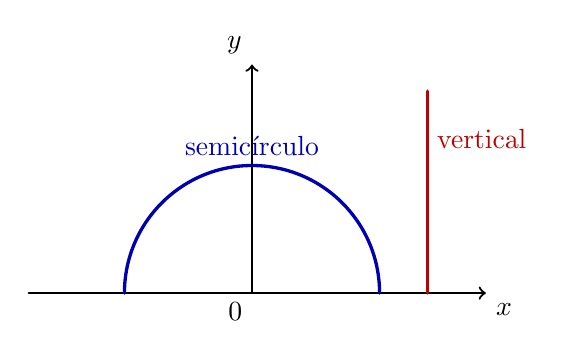
\begin{tikzpicture}[scale=1.35,line cap=round]
  \draw[->,thick] (-2.1,0) -- (2.2,0) node[below right] {$x$};
  \draw[->,thick] (0,0) -- (0,2.15) node[above left] {$y$};
  \draw[blue!70!black,very thick] (-1.2,0)
    arc[start angle=180,end angle=0,radius=1.2cm];
  \draw[red!75!black,very thick] (1.65,0) -- (1.65,1.9);
  \node[blue!70!black,above] at (0,1.2) {semicírculo};
  \node[red!75!black,right] at (1.65,1.45) {vertical};
  \node[below left] at (0,0) {$0$};
\end{tikzpicture}
